\documentclass[10pt,a4paper]{article}
\usepackage[utf8]{inputenc}
\usepackage{amsmath}
\usepackage[margin=1.2in]{geometry}
\usepackage[pdftex]{graphicx}
\usepackage{amsfonts}
\usepackage{amssymb}
\usepackage{hyperref}
\hypersetup{
    colorlinks=true,
    citecolor=black,      
    urlcolor=cyan,
}
\usepackage[T1]{fontenc}
\renewcommand*{\figurename}{Rys.} 
\renewcommand*{\tablename}{Tab.} 
\author{Rafał Kornel}
\title{\textbf{Badanie własności elementów półprzewodnikowych - diod.}}
\date{}
\begin{document}
\maketitle

\section*{Abstrakt}
W niniejszym doświadczeniu zostały przebadane charakterystyki prądowo-napięciowe elementów półprzewodnikowych - diod. Przebadane zostały diody krzemowa oraz LED. W tym celu zostały skonstruowane obwody elektryczne i przy użyciu oscyloskopu wykreślone zostały charakterystyki prądowo-napięciowe. Na ich podstawie dopasowano zależność teoretyczną, obliczono wartość $I_G = 0.3 \pm 2.1 \text{$\mu$A}$. Udało się potwierdzić przewidywania modelu teoretycznego, ponadto oszacowano napięcia przewodzenia diody krzemowej: $U_{Si} \approx 0.19 \pm 0.1 \ \text{V} $, oraz diody LED: $ U_{LED} \approx 1.6 \pm 0.3 \ \text{V} $. Wyznaczono krytyczną częstotliwość migania diody LED na $f = 33 \ \text{[Hz]}$.

\section*{Wstęp teoretyczny}
Diody, w szczególności krzemowe, germanowe, LED oraz Zennera są elementami elektrycznymi nieliniowymi, tzn takimi, których charakterystyka prądowo-napięciowa nie jest funkcją liniową. Ponadto, wyżej wymienione diody są elementami półprzewodnikowymi, czyli złożonymi z materiałów półprzewodnikowych. Takimi materiałami są pierwiastki z grupy 14 układu okresowego, lub związki / domieszki pierwiastków z grup 13-15. W przypadku diody krzemowej mamy do czynienia z kryształem krzemu, domieszkowanym atomami z grupy 15 po jednej strony (złącze n - negative), oraz po przeciwnej stronie atomami z grupy 13 (złącze p - positive). Tak przygotowany materiał nazywamy złączem p-n. Jedną z najważniejszych cech diod jest asymetryczność polaryzacji: jeśli przyłożymy napięcie zgodnie z polaryzacją, to prąd nie będzie płynął przez złącze, jeśli przeciwnie, to umożliwimy przepływ. Charakterystyka prądowo-napięciowa dana jest przez równanie Shockley'a:
\begin{equation}
I(U) = I_G[\text{exp}(\frac{eU}{Mk_BT}) - 1 ]
\end{equation},
gdzie $I_G$ to prąd generacji, zależny od właściwości materiału oraz od domieszkowania, $e$ to ładunek elektronu, $k_B$ to stała Boltzman'a, $T$ to temperatura, $M$ to stała związania z rodzajem półprzewodnika, a $I$ oraz $U$ to kolejno natężnie prądu płynącego przez diodę, oraz spadek napięcia na tejże.
Możemy tę zależność odwrócić, dostajemy wtedy:
\begin{equation}
U(I) = \frac{Mk_BT}{e}\text{ln}(\frac{I}{I_G} + 1) 
\end{equation}
W dalszej części będziemy posługiwać się wzorem (2).

Dioda LED jest elementem bardzo podobnym do diody krzemowej, jedyną istotną różnicą jest fakt, iż dioda LED (light emiting diode) emituje promieniowanie w zakresie widzialnym. Możemy zatem zaobserwować, kiedy przez diodę przepływa prąd. 


\section*{Przebieg doświadczenia}
Do badania charakterystyk prądowo-napięciowych zostały skonstruowane obwody elektryczne. Pierwszym krokiem doświadczenia było zidentyfikowanie rodzaju diod. Został do tego użyty miernik uniwersalny Brymen 805. 
Po poprawnym sklasyfikowaniu diod został przygotowany następujący układ, przedstawiony na Rys.\ref{uklad_1}.
\begin{figure}[ht!]	
	\begin{center}
		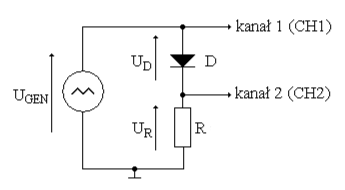
\includegraphics[width = 0.6\textwidth]{obwod1.png}
		\caption{Schematyczny rysunek przedstawiający obwód służący do wykonania pomiarów napięcia w celu zbadania charakterystyki prądowo-napięciowej diody krzemowej.}
		\label{uklad_1}
	\end{center}
\end{figure}	
Składał się on z następujących elementów: 
\begin{itemize}
\item Generatora funkcji prądu zmiennego
\item Diody krzemowej $D$
\item Opornika $R$
\end{itemize}
Spadek napięcia na diodzie, czyli $U_D$, oraz na oporniku $U_R$ odczytywane były z oscyloskopu.
Dzięki niemu możliwe było zmierzenie napięć $U_R$ oraz $U_D$ w punktach o równej fazie, które pozwoliły wyznaczyć charakterystykę prądowo-napięciową diody krzemowej.
Kolejnym krokiem doświadczenia było skonstruowanie obwodu pokazanego na Rys.\ref{uklad_2}.

\begin{figure}[ht!]	
	\begin{center}
		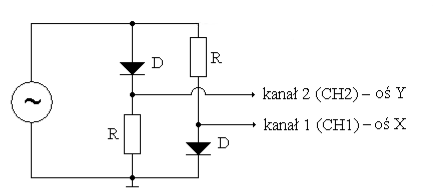
\includegraphics[width = 0.6\textwidth]{obwod2.png}
		\caption{Schematyczny rysunek przedstawiający obwód służący do badania charakterystyki prądowo-napięciowej diody krzemowej za pomocą 
		oscyloskopu.}
		\label{uklad_2}
	\end{center}
\end{figure}	

Jest on analogiczny do poprzedniego obwodu, również składa się z diod i oporników. Po podłączeniu dwóch żył do dwóch kanałów na oscyloskopie (tak jak na schemacie), przełączono oscyloskop w tryb pracy XY, czyli na osi X rysował on sygnał z gałęzi prawej, a na osi Y z lewej. To pozwoliło na wyrysowanie charakterystyki diody bezpośrednio na oscyloskopie, oraz wyznaczenie napięcia przewodzenia.
Następnym krokiem doświadczenia było skonstruowanie identycznego jak na schemacie poprzednim (Rys.\ref{uklad_2}) obwodu, z zamianą diod krzemowych na diody LED. Pozwoliło to zaobserwować charakterystykę prądow-napięciowa diody LED, oraz oszacować napięcie przewodzenia.
W ostatnim kroku doświadczenia wyznaczony krytyczną częstotliwość migania diody LED. Zmiana częstotliwości prądu wejściowego pozwoliła zaobserwować zmianę częstotliwośći migania diody, oraz moment, w którym ludzkie oko nie odróżnia już pojedynczych impulsów.

\section*{Analiza danych}
\subsection*{Dioda krzemowa}
Wychodząc od Rys.\ref{uklad_1} możemy zauważyć, że kanał 1 (CH1) na oscyloskopie pokazuje całkowity spadek napięcia na układzie, a kanał 2 (CH2) spadek napięcia na oporniku. Kanał 2 zatem pokazuje napięcie, po przejściu przez diodę, zaś kanał 1 przed. Możemy zatem mając te dwa napięcia wyznaczyć spadek napięcia na diodzie, 
\begin{equation}
U_D = U_{GEN} - U_R,
\end{equation} 
oraz znając opór $R$ i korzystając z prawa Ohm'a dla opornika, natężenie prądu płynącego w układzie,
\begin{equation}
I_D = \frac{U_R}{R}
\end{equation}
Wartości zmierzonych oporów oraz spadków napięć na diodzie, które służyły do rozpoznania rodzajów diod znajdują się w Tab.(\ref{opory}).

\begin{table}[htp!]
\begin{center}
\begin{tabular}{|c|c|}
\hline
$D_{Si}$ 					  & 0.569 {[}V{]}					  \\
$D_{LED}$                      & 1.63 {[}V{]}                       \\
$D_Z$                          & 1.9 / 0.728 {[}V{]}                \\
$D\_\{Ge1\}$                   & 0.33 {[}V{]}                       \\
$D\_\{Ge2\}$                   & 0.296 {[}V{]}                      \\
$R_1$                          & 1.00082 k$\Omega$                  \\
$R_2$                          & 1.00588 k$\Omega$                 \\
\hline
\end{tabular}
\end{center}
\caption{Zmierzone wartości oporów oraz spadków napięć na elementach układu. Oznaczenia subskryptów: $Si$ - krzemowa, $LED$ - świecąca, $Z$ - Zennera, $Ge1/2$ - diody Germanowe,  $R_{1/2}$ - oporniki.}
\label{opory}
\end{table}
Teraz korzystając ze wzorów (3) oraz (4) możemy wyznaczyć charakterystykę prądowo-napięciową diody, zgodnie ze wzorem (2).
\begin{figure}[ht!]	
	\begin{center}
		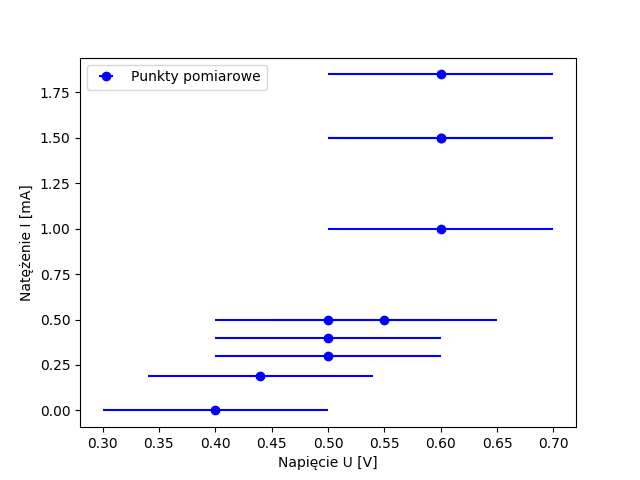
\includegraphics[width = 0.6\textwidth]{i_u.png}
		\caption{Punkty pomiarowe naniesione na wykres.}
		\label{i_u}
	\end{center}
\end{figure}	
\begin{table}[htp!]
\begin{center}
\begin{tabular}{|c|c|c|c|}
\hline 
$U_{GEN}$ [mV] & $U_R$ [mV] & $U_D$ [mV] & $\sigma$ [mV] \\ 
\hline
\hline
400 & 0 & 400 & 100 \\ 
\hline 
630 & 190 & 440 & 100 \\ 
\hline 
900 & 400 & 500 & 100 \\ 
\hline 
1050 & 500 & 550 & 100 \\ 
\hline 
1600 & 1000 & 600 & 100 \\ 
\hline 
2100 & 1500 & 600 & 100 \\ 
\hline 
2450 & 1850 & 600 & 100 \\ 
\hline 
2100 & 1500 & 600 & 100 \\ 
\hline 
1000 & 500 & 500 & 100 \\ 
\hline 
800 & 300 & 500 & 100 \\ 
\hline 
\end{tabular} 
\end{center}
\caption{Tabela zmierzonych wartości napięć, wraz z niepewnościami.} 
\label{tab1}
\end{table}
Na Rys.\ref{i_u} można zobaczyć naniesione na wykres punkty pomiarowe. Widać niestety, że dla ustalonej wartości napięcia dostajemy kilka wartości natężenia (w dwóch przypadkach). Jest to problem wynikający z metody pomiaru, która opierała się na odczytaniu z oscyloskopu wartości napięcia wprost z wykresu, zamiast korzystając z wbudowanych funkcji oscyloskopu. Z tego samego powodu również niepewności pomiarowe są tak duże. Aby pozbyć się tego problemu, który mógłby uniemożliwić znalezienie dopasowania funkcyjnego, zależność została odwrócona, zatem zamiast szukać funkcji $I(U)$ znaleziona została funkcja $U(I)$. Ponadto, został usunięty jeden punkt pomiarowy, aby pozbyć się problemu opisanego wyżej, był to pomiar $U_{gen}$ = 1000 mV. W takim układzie punkty pomiarowe, razem z niepewnościami oraz dopasowaniem funkcji (2) znajduje się na Rys.\ref{u_i}.
\begin{figure}[ht!]	
	\begin{center}
		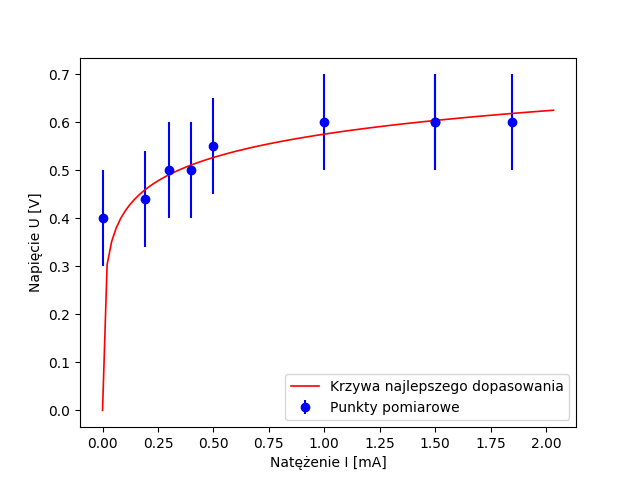
\includegraphics[width = 0.6\textwidth]{u_i.png}
		\caption{Punkty pomiarowe naniesione na wykres, razem z niepewnościami oraz dopasowaniem funcyjnym, danym wzorem (2).}
		\label{u_i}
	\end{center}
\end{figure}	
Współczynniki dopasowania są następujące:
$$ \frac{Mk_BT}{e} = 70 \pm 68 \ \text{[mV]}$$
$$ I_G = 0.3 \pm 2.1 \ \text{[$\mu$A]} $$
Widać, że natężenie prądu generacji $I_G$ jest bardzo małe, w porównaniu do prądów płynących przez układ, w istocie jest o trzy rzędy wielkości mniejsze. Rezultat taki jest zrozumiały, jeśli przypomnimy sobie fakt, iż prąd generacji $I_G$ jest związany z samorzutnym przepływem nośników prądu przez złącze p-n. \\
Następną część doświadczenia stanowiło wyrysowanie na ekranie oscyloskopu, przy użyciu funkcji X-Y charakterystyki prądowo-napięciowej bezpośrednio, dzięki układowi z Rys.\ref{uklad_2}. Pokazało to kształt funkcji $I(U)$ taki, jaki oczekujemy, czyli eksponencjalny. Na podstawie tego wykresu zostało oszacowane napięcie przenoszenia, czyli wartość napięcia przyłożonego do diodu, przy którym obserwujemy znaczne zwiększenie przepływu prądu przez tenże element. Oszacowana wartość wynosi 
$$ U_{Si} = 190 \pm 100 \ \text{[mV]} $$.
Jest ono rozbieżne z napięciem przenoszenia zmierzonym przy użyciu miernika uniwersalnego, które wynosi $U_{Zm-Si} = 569 \ \text{[mV]}$. Można to wyjaśnić tym, iż przy badaniu tejże charakterystyki, skala na osiach była zbyt mała, przez co to co wyglądało na znaczny wzrost natężenia, tak naprawdę nim nie było.

\subsection*{Dioda LED}
Po zbadaniu charakterystyki diody krzemowej, zbadano charakterystykę diody LED. Po skonstruowaniu układu z Rys.\ref{uklad_2}, lecz stosując diody LED można było znów skorzystać z funkcji X-Y oscyloskopu i zbadać charakterystyke. Jej kształt analogiczny był do kształtu charakterystyki diody krzemowej, jedyną różnicą było przesunięcie wykresu w dodatnią stronę osi OX, czyli napięcie przenoszenia znajdowało się w innym miejscu. Oszacowano je na 
$$ U_{LED} = 1.6 \pm 0.3 \text{[V]} $$. 
Tym razem pomiar oszacowany pokrywa się z wartością zmierzoną, która wynosi $U_{Zm-LED} = 1.9 \text{[V]}$. Może to wynikać z tego, iż tym razem zastosowano poprawną skalę, przez co można było zauważyć faktyczne znaczne zwiększenie natężenia. \\
Po poprawnie wykonanej analizie charakterystyki zmierzono częstotliwość prądu, przy której ludzkie oko przestaje rozróżniać miganie diody. Wykonano dwa pomiary, jeden ustalając wysoką częstotliwość i stopniowo ją zmniejszając, aż do momentu zaobserwowania migotania diody, oraz drugi ustawiając niską częstotliwość i zwiększając ją, aż to zaobserwowania zaniknięcia migania.
$$ f_{-} = 32 \pm 1 \ \text{[Hz]}, \qquad f_{+} = 34 \pm 1 \ \text{[Hz]} $$, gdzie $f_-$ to częstotliwość krytyczna przy zmniejszaniu, zaś $f_+$ to częstotliwość krytyczna przy zwiększaniu częstotliwości.
Niepewność została ustalona na podstawie wykorzystanej rozdzielczości generatora funkcji.
Pomiary te pokrywają się dla częstotliwości równej $f = 33 \ \text{[Hz]}$, co ustalamy za graniczną częstotliwość migotania (cff - critical flicker frequency).

\section*{Podsumowanie}
W powyższym doświadczeniu udało się potwierdzić kształt charakterystyki prądowo-napięciowej, który zapewnił model teoretyczny. Wykorzystano do tego funkcje X-Y w oscyloskopie, oraz prostownik połówkowy (Rys.\ref{uklad_1}). Niewystarczająco dokładne okazały się jednak współczynniki wynikające z dopasowania modelowego, co oznacza, iż na podstawie pomiarów możemy rzetelnie oszacować jedynie rząd wielkości tychże wartości. Prąd generacji okazał się być o trzy rzędy wielkości mniejszy, niż prąd płynący w obwodzie, co wydaje się być sensowne. Na podstawie wykresu X-Y na oscyloskopie oszacowano wartości napięcia przenoszenia, jednak jedynie w przypadku diody LED udało się to zrobić z zadowalającym rezultatem. Dla diody krzemowej wynik nie pokrywał się ze zmierzoną wartoscią. Na koniec zmierzono graniczną częstotliwość migania, którą potrafi zaobserwować ludzkie oko, wynosi ona $f = 33 \ \text{[Hz]} $.


\end{document}